\documentclass[../dejiny-rodu-prusiku.tex]{subfiles}

\begin{document}

% str 75 @ 90
\section{Odnož Hodyně - větve Výrov}

Potomci Matěje Prusíka, výrovského rodáka ,usazeného v Hodyni.

1818 - 1900

Šestým dítětem výrovského rychtáře Vojtěcha Prusíka a jeho ženy Anny byl syn Matěj. Narodil se ve statku „u Boudů“ 22. 2. 1818. Byl to od dětství velmi nábožný člověk a ve svém domově, kde pomáhal až do svých 25, let byl spokojen. Teprve když jeho bratr Václav se 30. led­na 1843 oženil, začalo se uvažovati o tom, aby i on nezůstal svobodný a usadil se třeba v jiné blízké vesnici. Když se ve Výrově dozvěděli, že v Hodyni je na prodej usedlost č. 17, kde tehdy hospodařil Jan Tischer, byl tento statek zakoupen. S pomocí rodičů koupil jej Ma­těj Prusík se svou nastávající družkou života Annou Fakanovou z Hodyně. Stalo se to 3. 11. 1843. Usedlost tato mívala do roku 1805 číslo 10. Až do roku 1830 byla jejím majitelem rodina Janečků. Je zajímavé, že v roce 1782 hospodařil zde Adam Janeček, který měl za ženu Barboru Prusíkovou, narozenou 6. 5. 1756 v Sedlci. A tu, počátkem listopadu 1843 dostává se sem hrou osudu opět člen našeho rodu, Matěj Prusík z Výrova. Usedlost byla koupena za 2.800.- zlatých.

V Hodyni dnes žije asi 140 lidí. Samozřejmě, před 125 lety bylo jich tam méně. Ves tato, ležící blíže Kralovického potoka, patřila zpočátku komoře královské, ale kolem roku 1220 dostala se klášteru plasskému směnou za Všehrdy. Průběhem mnoha staletí byli majiteli obce různí šlechtici jako Hanuš Kolovrat na Krasové, nebo Jan z Gutštejna na Nečtinách a částečně byl zde majetníkem i proslulý Florian Gryspek na Kaceřově. Ve vsi bývala výsadní rychta a v do­bě, kdy majetníkem byl klášter Plasy, a ten Hodyni měl nej­déle, robotoval mimo rychtáře každý sedlák. V této malé, půvabné vesničce u Kralovic narodila se Prokopu Fakanovi a Anně Jindříškové z Kočína 11. 7. 1820 dcera Anna. Tu si tedy vzal za manželku Matěj Prusík. Bylo to 28. 11. 1843. Od toho dne byl tedy usedlý rod Prusíků v Hodyni. Anna Pru­síková, rozená Fakanová zemřela ve svých 47 letech na psotník 21. 11. 1867.

Matěj Prusík se svou ženou Annou měli mnoho dětí, ale dospělo jen pět synů. Všechny jejich dcery, Barbora, Marie, Anna a Josefa předčasně v dětství zemřely. Matěj Prusík byl konservativnějším hospodářem než jeho bratr Václav a to se projevovalo i v jeho vlastním životě. Tak například zrcadlo znamenalo pro něho marnost a po celý život se do něho nepodíval. Byl to velmi dobrosrdečný muž a v jeho statku byl každý vždy upřímně vítán. On zemřel jako poslední ze čtyř bratrů Prusíků, narozených ve Výrově "u Boudů". Dožil se 82 let. Žil spokoje­ně na výměnku přes třicet let, když na usedlosti hospo­dařil samostatně již jeho prvorozený syn Vojtěch. Matěj Prusík zemřel na marasmus 17. 10. 1900.

% str 76 @ 91
Nejstarší syn Matěje a Anny byl Vojtěch Prusík, narozený 11. 4. 1847. Zemřel v Hodyni 31. 12. 1924. Stal se dědicem gruntu. - Další byl Josef narozený 20. 3. 1849. Ve svých dvaceti letech se vystěhoval do Ameriky, za­ložil tam četnou rodinu a zemřel 4. 8. 1927. Na své farmě u Shawano ve státě Wisconsin v USA dokončil svůj život. Do své vlasti se již nikdy nevrátil.

Třetí syn byl Václav. Narodil se 13. 8. 1853, usadil se v blízkých Kozojedech a zemřel tam v krásném věku 90 let 28. 7. 1943. - Čtvrté dítě Matěje a Anny byl František Prusík. Narodil se 14. 3. 1857, usadil se nakonec v Lounech, kde byl skladníkem v cukrovaru a tam zemřel 1. 8. 1941. Poslední byl Jan Prusík, nar. 25. 5. 1859. Byl u finanční stráže a působil dlouho v Hrádku nad Nisou a zvláště v Kőnigshahnu /Královec/ u Žacléře. Zemřel v Praze u svého syna 26. 10. 1937.

Prvním synem jak jsme již uvedli, byl Vojtěch Prusík. Narodil se na statku v Hodyni č. 17 dne 11. 4. 1847. Vystudoval šest tříd gymnasia v Plzni, ale když jeho maminka Anna roz. Fakanová tak brzy zemřela, studia svá již nedokončil a vrátil se domů, kde převzal po otci usedlost. Jeho otec Matěj se již znovu neoženil. Vojtěch Prusík byl velmi inteligentním sedlákem. Dlouho byl starostou obce Hodyně, také jeden čas byl čle­nem Okresního výboru v Kralovicích. Po velké přírodní katastrofě v devadesátých letech minulého století, kte­rá také téměř zničila celou úrodu v Hodyni, byl vyslán s jinými delegáty z okolních obcí k císaři do Vídně, s prosbou o pomoc. Protože dovedl německy, stal se tam mluvčím této deputace. Rád citoval výrok císaře Františka Josefa I., který mu při odchodu od audience řekl česky: „Ti s Pohem a já Ti pudu nápomocen". - Vojtěch Prusík podporoval rád vše nové co se uvádělo v hospodařeni, ať to bylo hnojení, nové nářadí či stroje. Jako již před tím jeho strýc Václav Prusík ve Výrově začal sekati obilí kosou místo srpem, i on šel příkladem vstříc v Hodyni. Jako ve Výrově byli zpočátku nedůvěřiví, tak i v Hodyni následovali ostatní zemědělci Vojtěchova příkladu až za rok po něm.

Vojtěch Prusík vyvolil si za družku svého života Annu Jánskou z Dřevce. Narodila se tam 28. 1. 1851, ale tak jako Vojtěchova maminka Anna i jeho manželka Anna zemřela poměrně mladá. Bylo jí 41 let když zemřela v Hodyni na zánět pobřišnice 24. 1. 1892. Vojtěch se svou ženou měli dvanáct dětí. Dospělo jich sedm. Měli tři dcerky se jménem Marie, které zemřely v dětství a teprve čtvrtá, pokřtěná tímto jménem, dospěla. Také jejich dvojčata Cyril a Anna, zemřela, když jim byl jeden rok. Vojtěch Prusík oženil se začátkem XX. století   znovu a to s Marii Štěpánovou ze Dřevce. Toto manželství již bylo bezdětné. Marie Prusíková, druhá žena Vojtěchova, zemřela v Hodyni 4. 12. 1939.
Usedlost č. 13, která patřila rodině Fakanů a odtud pocházela žena Matěje Prusíka, byla v roce 1871 prodána
% str 77 @ 92
kováři Janu Kožíškovi za 1170 zlatých, ale jen s částí pozemků. Ostatní pole a louky přešly na Vojtěcha Prusíka, takže tím si zvětšil výměru. Po smrti své matky vyplatil Vojtěch Prusík každému bratru a nebo zaručil jim podíly p0 200 zlatých. První podíl vybral hotově jeho bratr Josef, který emigroval do Ameriky. Vojtěch Prusík byl v Hodyni vážený a oblíbený a to nejen proto, že býval starostou, ale i pro svou dobrosrdečnou a pohostinnou povahu. Zemřel na výměnku na zápal plic dne 31. 12. 1924.

Vojtěch Prusík se svou ženou Annou měl těchto sedm dětí: Nejstarší byla dcera Františka nar. 7. 4. 1870. Ta se stala dědičkou usedlosti č. 17, kde se odedávná říkalo „u Laibů“ a v roce 1912 zakoupila se svým mužem Františkem Hanzlíčkem, rodákem z Obory u Kaznějova, pěkný dvůr Machkův, a ten také později předala svému bratru Vojtěchovi. Manželství Františky Hanzlíčkové, roz. Prusíkové bylo bezdětné. Její muž byl sice bystrým, sčetlým člověkem, ale hospodář to nebyl vynikající. Hlavní tíhu nesla jeho žena. Františka Hanzlíčková zemřela 27. 1. 1938. Druhé dítě, které dospělo, byl syn Václav. Narodil se 6. 12. 1873, stal se strojvůdcem na dráze, mnoho let byl usazen v Plzni a zemřel v Třemošné 3. 3. 1938. Třetí byla Anežka provdaná  Kasalová. Narodila se 1. 3. 1878 a zemřela 24. 7. 1928. Druhým synem Vojtěcha Prusíka z Hodyně byl Josef. Narodil se 30. 10. 1879, působil jako úředník u dráhy a zemřel tragicky v květnu 1945 blíže Walczu v nynějším Polsku, když již věznice v Golnowě, kde byl zavřen, byla osvobozena. - Další byl František Prusík, narozený 23. 8. 1881 v Hodyni, byl majitelem drogerie a zemřel v Hodyni, kde se usadil ke konci života 31. 12. 1959. Šestým dítětem Vojtěcha Prusíka  z Hodyně byl syn Vojtěch. Narodil se 21. 3. 1888, hospodařil po své sestře Františce Hanzlíčkové v Hodyni a zemřel 18. 8. 1948. Poslední je dcera Marie, narozená 22. 9. 1890. Poprvé provdala se za učitele Ladislava Vodáka. Vzala si ho v roce 1914, ale po deseti letech bylo toto manželství rozloučeno.

Žila s ním v Čivicích a Kožlanech. V roce 1930 se znovu provdala za úředníka drah Františka Bílka a nyní jako vdova žije v Praze 7, Na Maninách č. 32. Delší čas žila také u své sestry Anežky, provdané Kasalové, kterou také ošetřovala do její předčasné smrti.

K Marii Bílkové, roz. Prusíkové, která zůstala bezdětná, obracejí se často s důvěrou četní její synovci a neteře i další jejich potomci, jako k poslednímu členu rodiny Vojtěcha Prusíka z Hodyně. Zemřela 31. 12. 1974.

Prvním synem Vojtěcha Prusíka a Anny roz. Jánské v Hodyni, který dospěl, byl Václav.  Narodil se 6. 12. 1873. Studoval krátce na gymnasiu v Klatovech. Tam však prováděl všelijaké nedobré kousky. Prodal, ačkoliv nouzí netrpěl, jako student, peřinu. A když se ukázalo, že soustavné učení a vysedávání ve škole se mu nelíbí, byl dán na učení zámečnictví. Toto řemeslo si oblíbil a stal se později velmi schopným strojvůdcem drah. Prvním jeho působištěm byly Karlovy Vary. Pak byl přeložen do Rakovníka a největší část života strávil v Plzni. Vzal si za manželku Marii
% str 78 @ 93
Němcovou, nar. 25. 3. 1882 v Plzni. Měli pět dětí. Václav Prusík zemřel ve své vilce v Třemošné, kde žil na pensi, 3. 3. 1938 a byl pochován v Plzni. Jeho žena Marie přežila ho jen o rok, zemřela v Třemošné 21. 6. 1939.

Nejstarší dítě Václava Prusíka a Marie, byla dcera Milada. Narodila se v Karlových Varech 19. 7. 1900. Několik let žila také v Praze a později provdala se za obchodníka Václava Langa a bydlí dnes v Plzni, Divadelní 4. Milada Langová, rozená Prusíková má čtyři děti. Její syn Václav Lang narodil se 16. 10. 1926. Je stavebním technikem a bydlí v Plzni, Škrétova 43. Má dvě děti. Dcera Libuše nar. 19. 12. 1952 a synek Václav nar. 24. 5. 1961. Druhá byla dcera Marie, nar. 22. 9. 1927. Její dcera Alena Langová je nemanželská. Narodi­la se 19. 12. 1949.

Marie Langová provdala se pak jako Bobková a měla ještě další dvě dcerky. Jindřiška Bobková narodila se 21. 11. 1954 a Marie Bobková narodila se 22. 2. 1956. Jejich maminka Marie Bobková zemřela mladá na rakovinu 1. 7. 1956. Sirotků ujala se obětavě babička s dědečkem a vychovali je. - Další je dcera Milada, provdaná Martinková. Narodila se 28. 10. 1934, je zdravotní sestrou a je bezdětná. Bydlí v Plzni, Tomanova 5 a zvláště ona stará se obětavě o děti své předčasně zemřelé sestry Marie. - Posledním dítětem Milady Langové je dcera Josefa. Narodila se 5. 3. 1939. Bydlí v Plzni, Kollárova č. 5. Má synka Václava Zunu, jak je jeho matka provdaná. Narodil se 8. 2. 1959.

Dalším synem strojvůdce Václava Prusíka rodáka z Hodyně byl Václav. Narodil se v Plzni 1. 4. 1902, byl šoférem pošty v Praze, ale brzy onemocněl a zemřel na souchotiny v mladém věku 24 let, 1. 4. 1926. Je pochován v Plzni. Další byl syn Ervín Prusík. Narodil se 20. 8. 1904 v Rakovníce. Vyučil se drogistou u svého strýce Františka Prusíka, měl pak svou drogerii  v Chudenicích u Klatov a v Plzni, ale v tomto podnikání se mu příliš nedařilo. Naposledy byl spolumajitelem továrny na mýdlo v Praze - Libni pod firmou Prusík a spol., ale ani zde neuspěl. Jeho manželkou se stala Marie Jirásková, nar. 18. 5. 1903. Ervín Prusík zemřel v mladém věku 38 let, 5. července 1942 a je pohřben v Plzni. Vdova po něm, Marie Prusíková bydlí v Praze – Košířích, Holečkova 52. Ervín se svou ženou Marií měli spolu jediného syna, Ervína. Narodil se 11. 5. 1934 v Plzni. Měl v sobě talent na cizí jazyky, ale nemohl se stále uchytit na místě, kde by mohl uplatnit své schopnosti. Nějaký čas byl zaměstnán jako mechanik, ale to ho nebavilo. Toužil po světě. Jednoho dne v roce 1953 odešel ještě s několika kamarády ilegálně přes hranice do Rakouska a odtud dostal se po svízelném putování nakonec do USA. Počátky tam měl těžké, jako snad každý, ale nyní se tam již velmi dobře uplatnil jako úředník v pojišťovně a současně jako výpočtový technik v jednom průmyslovém podniku. Bydlí u New Yorku v New Foundland 11, Midlesex Court New Yersey. Jeho manželkou
% str 79 @ 94
je Francouzka roz. Monika Guiffantová 21. 8. 1931 v Brestu v Bretani. Ervín a Monika nemají zatím děti. Monika pracuje také jako úřednice. S Ervínem postavili si pěkný domek na sever od New Yorku v lesnatém a jezernatém kraji u Wanda—lake. Z kamarádů, kteří s Ervínem kdysi opustili svou vlast, žije ještě pouze jeden jako Ervín v USA. Ostatní jsou roztroušeni jinde po světě.

Další dítě Václava Prusíka, rodáka z Hodyně, je syn Karel. Narodil se 8. 9. 1907, v Plzni. Vyučil se v koloniálním obchodě, také kdysi u známé velké pražské lahůdkářské firmy Dřevo. Kratší dobu měl v tomto oboru i svůj podnik. Naposledy byl revisorem Krajské správy restaurací a jíde­len v Plzni. Za manželku vzal si Hermu Echtnerovou, která se narodila 27. 3. 1911 v Nýřanech u Plzně. Karel Prusík se svou ženou Hermou mají dvě děti. Bydlí v Plzni, Zámečnická 32. Jejich syn Václav Prusík narodil se 28. 9. 1933, vyučil se fotografem a v tomto oboru je stále zaměstnán v Plzni. Jeho manželkou je Jitka Hoblová, nar. 12. 10. 1936 ve Starém Plzenci. Tam také manželé bydlí v Nerudově uli­ci 766. Mají dvě děti. Syn Václav Prusík nar. 27. 12. 1960 a dcerka Jitka narozená 8. 5. 1964. Václav Prusík patří k těm mladým lidem u nichž to není zdaleka pravidlem, kte­ří se mimořádně zajímají o historii rodu, k němuž patří. Je vždy velmi ochotným pomocníkem v tomto našem historickém díle. - Dcera Karla Prusíka, Jana provd. Kudrová, narodila se 25. 1. 1940 v Plzni, má za manžela technika Josefa Kudru. Bydlí v Plzni, Čermákova 62. Mají spolu syna Pavla, narozeného 22. 5. 1964.

Posledním dítětem strojvůdce Václava Prusíka, je dcera Jarmila. Narodila se v Plzni 7. 3. 1910 a provdala se za úředníka drah, Jaromíra Fialu. Bydlí v Plzni, Čechurově, Zelenohorská 71. Má dvě dcery. Jarmila nar. 21. 9. 1936 je provdaná za důstojníka Pytlíka v Plzni, kde bydlí Na Slovanech, Šeříkova 30. Má dceru Ivanu nar. 25. 6. 1959. Druhá dcera Jarmily Prusíkové, provdané Fialové je Vlasta. Narodila se 21. 12. 1939 a provdala se za technika Škodovky, Kokošku. Bydlí v Plzni - Letné, Partyzánská č. 2. Vlasta Kokoškova má dva synky. Karel nar. 9. 11. 1963 a Petr nar. 20. 12. 1964.

Druhou dcerou Vojtěcha Prusíka a Anny v Hodyni byla Anežka. Narodila se 1. 3. 1878. Provdala se za poštovního zřízence J0sefa Kasala, který se narodil v r. 1864 ve Skořicích na Rokycansku. Usadili se spolu v Plzni a Anežka tak neměla příliš daleko do svého rodiště, Hodyně. Vždyť tam žil její tatínek ještě řadu let. Když její sestra Františka, provdaná Hanzlíčková zakoupila novou, lepší usedlost v Hodyni, zachránila Anežka Kasalová svoje rodiště, usedlost č. 17 v Hodyni, před tím, aby nepřišlo do cizích rukou. Statek, na němž se usadil v roce 1843 Matěj Prusík z Výrova, koupili v roce 1912 Kasalovi. Anežka Kasalová se svým mužem Josefem měli jediného syna Jaromíra. Ten se narodil 9. 2. 1899, vystudoval na plzeňské reálce a na pražské technice, elektrotechniku. Kratší čas působil ve Škodovce, ale pak až do důchodu byl zaměstnán v technickém referátě u pražské obce. Potomků po sobe nezanechal.

% str 80 @ 95
Se  svou ženou Julií, dcerou sochaře Piccardta, bydlili dlouho na Smíchově, U Nikolajky, a nyní po jeho prodeji bydlí na Smíchově, Nádražní 50. Jaromír Kasal lnul vždy k rodišti své matky, Hodyni a vůbec k celému rodu Prusíků. Jeho matka Anežka Kasalová, roz. Prusíková,  žila se svým mužem několik let v Krušovicich u Rakovníka, kde otec inženýra Jaromíra Kasala byl poštmistrem. Anežka zemřela v Praze ve svých padesáti letech. Bylo to 24. 7. 1928 a je pochována Malvazinkách. Její muž ji přežil o dvě leta.

Dalším dítětem Vojtěcha Prusíka z Hodyně byl syn Josef. Narodil se 30. 10. 1879 v Hodyni. Dostal se brzy k železnici a jeho prvním místem byly v roce 1904 Klatovy. Pak se dostal do Brodu nad Lesy, kde byl na nádraží až do roku 1930. Postavil si později pěknou vilku v Klatovech, Pod Hůrkou a odešel tam na pensi. Měl za manžel­ku Barboru, roz. Rádlovou, naroz. 23. 10. 1883 ze Štěnovic u Plzně. Ta zemřela v Klatovech 17. 4. 1952. Josef Prusík, jak se mu v rodině říkalo "signál" byl zatčen v roce 1944, odsouzen na jeden a půl roku pro pobuřující řeči proti Hitlerovi a vězněn v Golnowě u Štětina v Německu. Tam se sice dočkal osvobození v roce 1945, ale při ná­vratu do vlasti v květnu toho roku záhadně mizí jeho stopa. Podle svědků byl naposledy viděn u městečka Deutsche Krone v bývalých východních Prusích, dnes u Walcze v Polsku. Do vlasti se tedy již nevrátil. Bylo mu 66 let. Josef Prusík se svou ženou Barborou měli jedinou dceru, Libuši. Narodila se 4. 11. 1922 v Praze. Je dnes úřednicí na nádraží v Klatovech. Bydlí ve vilce, kterou postavili její rodiče v Klatovech, ul. čs. tankistů č. 364. Libuše, která se také vždy hlásí ke svému rodu, je dosud svobodná.

Pátým dítětem Vojtěcha Prusíka z Hodyně byl syn František. Narodil se 23. 8. 1881. Studoval krátce na gymnasiu v Klatovech, ale brzy se ukázalo, že nemá do studia mnoho chutí. Vyučil se pak v drogerii a svou velkou pílí a sympatickým vystupováním domohl se pěkného postavení. Měl svou vlastní, dosti velkou drogerii v Praze - Radlicích. Jeden čas měl ještě filiální drogerii v Radotíně. Za řadu let odcho­val ve svém podniku mnoho drogistů, kteří na něj rádi vzpomínali a dobře se v životě uplatnili s Prusíkovou školou. František Prusík byl hodně let členem ředitelství Občanské záložny na Smíchově. Od roku 1913 byl také členem obecního zastupitelstva na Smíchově, a to za bývalou stranu národně demokratickou. Na smíchovské radnici věnoval se zejména sociálním otázkám a chudinské péči a ta­ké v tomto směru vykonal mnoho pro ty nejpotřebnější. Z jeho popudu byla také vybudována lávka pro pěší nad smí­chovským nádražím. Jeho ženou byla Anna Grűnwaldová nar. 18. 2. 1876 v Jesenici u Prahy. Toto manželství zůstalo však bezdětné. František Prusík postavil si v pozdějším věku ve svém rodišti v Hodyni vilku na pozemku již zlikvidovaného statku č. 17, kde se narodil. Ke svému domovu se vždy rád vracel a proto bylo vždy jeho touhou, aby tam strávil konec svého života.

% str 81 @ 96
Konec jeho života nebyl utěšený, neboť jako statisíce živnostníků zůstal bez peněz po druhé světové válce a žil velmi skromně. Jeho žena Anna zemřela v Hodyni 12. 11. 1950. Shodou osudu zemřel František Prusík přesně za čtvrt století po svém otci, také na Silvestra a to 31. 12. 1959 v nemocnici v Plzni.

Posledním synem Vojtěcha Prusíka a Anny roz. Jánské, byl Vojtěch. Narodil se 21. 3. 1888 v Hodyni. Vojtěch Prusík užil do sytosti vojny. Prožil anexi Bosny a Hercegoviny v roce 1908 a pak byl v první světové válce na italské frontě. Tam utrpěl značná poranění, zvláště rukou. V roce 1921 se oženil s Leontýnou Konopáskovou z Hodyně, roz. 12. 10. 1892. Brzy pak předala mu sestra Františka Hanzlíčková statek, kde Vojtěch Prusík dobře hospodařil. Ještě však za svého života jej prodal. Z tohoto manželství narodily se dvě dcery. Vlasta nar. 5. 2. 1922 provdala se za úředníka města Plzně Jana Fialu. Bydlí v Plzni, Čechurově, Lomená 20. Mají dvě děti. Syn Jan Fiala nar. 4. 2. 1943 má dcerku Janu nar. 3. 9. 1967, dcera Vlasta provdaná Herinková nar. 27. 3. 1946 má dceru Evu nar. 28. 9. 1967. Všichni bydlí v téže vilce, až na Janu. Druhá dcera je Miluška, která se narodila 11. 3. 1925 v Hodyni a provdala se do Výrova č. 1 za sedláka Václava Vopata. Mají dvě děti. Dcera Miroslava nar. 5. 11. 1946 je provdaná Rodová a bydlí dnes ve vilce svého prastrýce Františka Prusíka v Hodyni. Má dcerku Miroslavu, nar. 12. 4. 1967. Syn Václav Vopat je narozen 16. 2. 1955. Vojtěch Prusík, žijící již na odpočinku, jehož však dlouho neužil, zemřel 18. srpna 1948. Byl pochován na kralovickém hřbitově. Vdova po něm, Leontýna Prusíková zemřela 10. 3. 1965.

\subsection{První Prusík usedlíkem v Novém světě}

Druhým synem Matěje Prusíka a Anny roz. Fakanové v Ho­dyni byl Josef. Narodil se 20. 3. 1849. Až do svých dva­ceti let pomáhal doma v hospodářství a když bylo rozhodnuto, že dědicem gruntu stane se prvorozený Vojtěch, uvažovalo se co počít s Josefem. Jeho matka tehdy již byla po smrti, grunt mu nebyl určen a po prusko-rakouské válce 1866, doby byly stále neklidné. V těch časech od­jíždělo do Ameriky mnoho Čechů i z Kralovicka. A tu se rozhodl Josef Prusík, že také bude hledat své štěstí za mořem. Začátkem roku 1869 rozloučil se se svými drahými a rodnou vesnicí a opustil vlast navždy. Počátkem února 1869 dojel do New Yorku a odtud se později dostal do přístavu Green Bay ve státě Wisconsin. Tam žil několik let a všelijak si vydělával na živobytí. Poznal tam také svou budoucí ženu Kateřinu. Narodila se 17. 9. 1858 jako Janková, také v Čechách. Její matka byla porodní babičkou a také ona se tomu naučila a to jí bylo velice užitečné, když později žila na americkém venkově se svým mužem a lékař byl nekonečno daleko. Za několik let odjel pak Josef Prusík se svou ženou Kateřinou do blízkosti městečka Shawano v témže státě. Tam se nakonec usadili na své farmě a hospodařili přes padesát let. Josef Prusík vždy rád vzpomínal, jako
% str 82 @ 98
ostatně všichni krajané američtí, a se svými bratry si až do konce života dopisovali. Byl to velký katolík a když po první světové válce jeho starší bratr Vojtěch přestoupil k církvi československé, ostře mu to vytýkal. Nikdo z jeho tři dětí, které dospěly, nechtěl však farmařit. Když již tato práce Josefa a Kateřinu neobyčejně zmáhala, prodal Josef svou farmu blízko Shawano a žil asi jen dva roky na odpočinku. Zemřel 4. 8. 1927. Jeho žena Kateřina ho přežila o 20 let, zemřela u jedné ze svých dcer 16. 11. 1947.

% str 81+1 @ 97
\begin{figure}
\centering
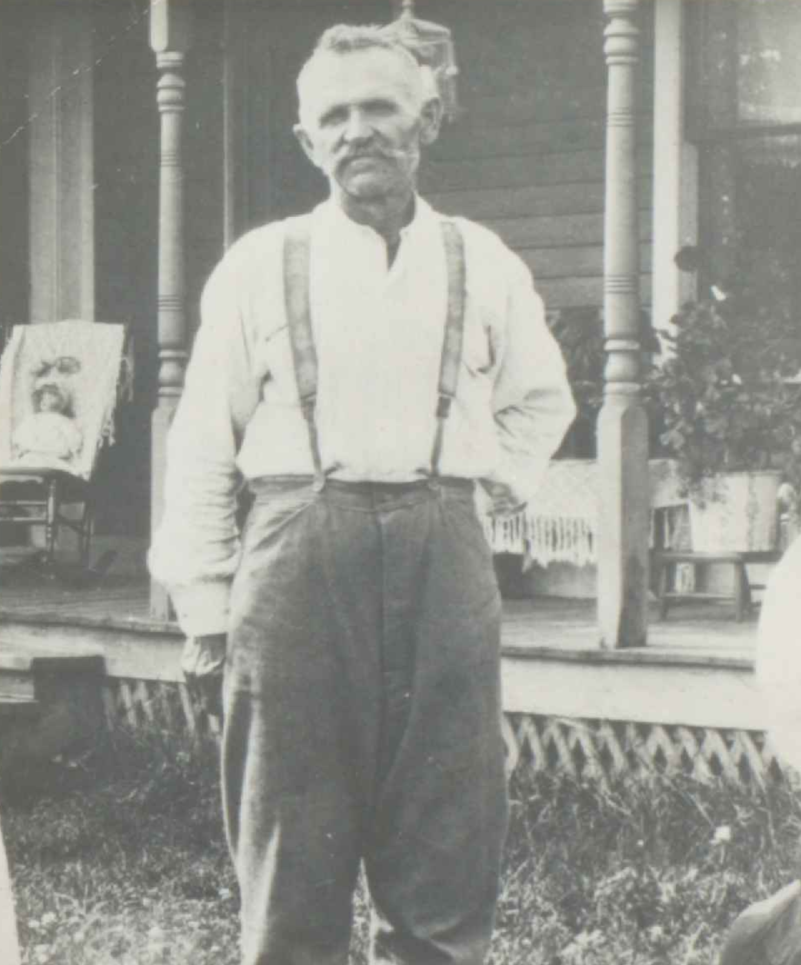
\includegraphics[width=\textwidth, height=\textheight, keepaspectratio]{097-a-josef_prusik_z_hodyne}
\caption{Josef Prusík z Hodyně (1849 – 1927), usazený jako první Prusík v USA v roce 1869}
\label{fig:097-a-josef_prusik_z_hodyne}
\end{figure}

\begin{figure}
\centering
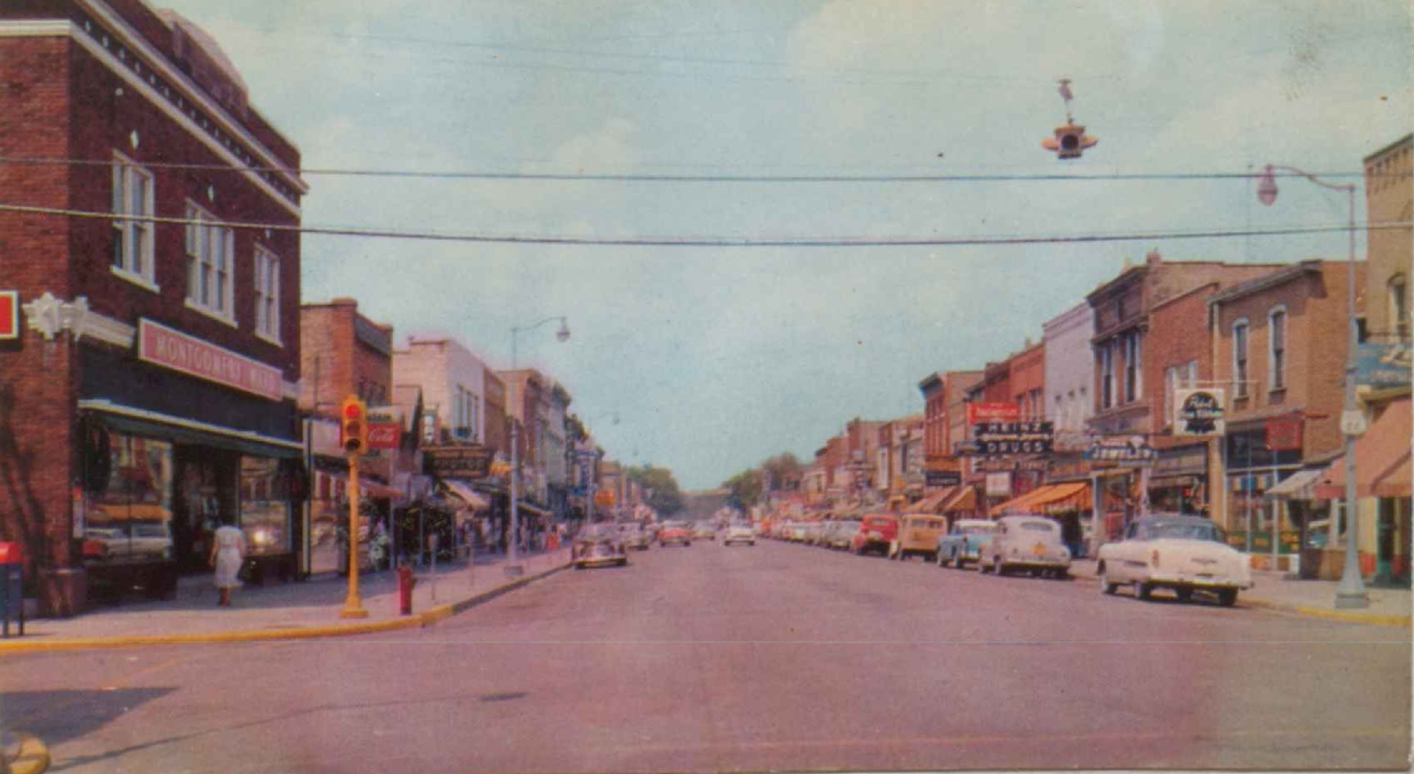
\includegraphics[width=\textwidth, height=\textheight, keepaspectratio]{097-b-mesto_shawano}
\caption{Město Shawano ve státě Wisconsin v USA, kde žijí potomci Josefa Prusíka z Hodyně}
\label{fig:097-b-mesto_shawano}
\end{figure}

% str 82 @ 98 (pokr.)
Josef Prusík a Kateřina, roz. Janková měli spolu šest dětí. Čeněk a Otylie zemřeli velmi záhy a Arnošt Prusík zemřel, když mu byly čtyři leta. Jediným jeho synem, který dospěl, byl Adolf. Narodil se 5. 12. 1881, pracoval v papírnách a žije dnes v Shawano na odpočinku, jako dnes nejstarší žijící Prusík na světě. - Dcera Ema narodila se 25. 10. 1892, provdala se za strojníka Jiřího Boehlera a žije ve městě Milwaukee ve státě Wisconsin. Druhá dcera Josefa Prusíka, Kateřina nar. 25. 11. 1895 prov­dala se za elektrotechnika Karla Radtkeho. Jako vdova žije dnes v Shawano. O osudech celé této rodiny povíme si nyní více.

Syn Josefa Prusíka, Adolf, přestože se narodil na farmě a od mládí musil pracovati na polích, neměl žádné chuti, trvale zakotviti v zemědělství. Stát Wisconsin je velmi lesnatý a tamní papírny skýtaly proto mnoho pracovních příležitostí a té také Adolf využil. Stal se dělníkem jedné takové papírny, po celý život tam jako dělník pracoval. Narodil se 5. 12. 1881 a patří dnes me­zi nejstarší osoby na světě s tímto jménem. Jiný Prusík, který by byl starší, není zatím jinde ve světě znám. Jeho manželkou stala se žena českého původu Otylie roz. Tatovská. Narodila se v Čechách 14. 12. 1883. - Adolf Prusík s Otylií měli spolu jednu dceru a čtyři syny. Všichni synové mají potomky se jménem Prusík, takže i za "velkou louží“ žijí dnes četní členové našeho rodu po meči i po přeslici. Jméno Prusík rozmnožili v odnoži Hodyně větve výrovské co nejvydatněji. Adolf Prusík se svou ženou Otylií žijí na odpočinku v Shawano, Maurer Street ve statě Wisconsin na severu USA.  Adolf Prusík zemřel 4. července 1969.

Nejstarším dítětem Adolfa Prusíka v USA je dcera Evelyn. Narodila se 29. 9. 1908 a byla dvakráte provdána, ne však šťastně. Vždy bylo její manželství rozvedeno z viny man­želovy. Dnes je Evelyn zaměstnána v hotelu Green Bay, Wisconsin a tam bydlí s dcerou Georgette v ulici Main Street, 328. Evelyn Prusíková byla po prvé provdána Schenková. Z tohoto manželství se jí narodili čtyři synové. Všichni pracují jako kvalifikovaní dělníci tzv. černého řemesla v různých továrnách ve státě Wisconsin. Nejstarší je Elmer Schenk. Narodil se 27. 4. 1926 a bydlí v Green Bay 2744, Whipponwill Drive. Má dvě děti. Jsou to Reyne Anna Schenková nar. 12. 3. 1951, a syn Robert nar. 1. 4. 1949. Druhým synem Evelyn roz. Prusíkové je Lyle Schenk nar. 7. 12. 1927. Bydlí ve městě Milwaukee, 17345, 65th Street. Má, jako

% str 83 @ 99
Jeho bratr Elmer také dvě děti. Jsou to chlapci, Alan nar. 15. 4. 1960 a Glenn Schenk, nar. 10. 7. 1956. Třetí­ je Dale Schenk. Narodil se 30. 3. 1930, má pouze jednoho synka. Je to Michal, nar. v březnu 1955. Poslední­m dítětem z prvního manželství­ Evelyn Prusí­kové je syn Eduard Schenk. Narodil se 5. 7. 1936 a zvláště on se hrdě hlásí k českému původu své maminky. Eduard má tři děti. Jsou to synové Daniel Schenk naroz. 17. 9. 1962, Štěpán nar. 5. 10. 1960 a dcera Stacy Sue Schenková nar. 10. 4. 1964. Děti bydlí­ se svými rodiči v pěkném vlastní­m domku v Green Bay 54301, 2634, Oakwood Drive. Green Bay je přístavní město­ a bydlí­ tam jak jeho matka, tak i bratr Elmer a sestra Georgette. Jeho bratři Lyle a Dale Schenkovi bydlí­ v městě Milwaukee. Adresa Dale Schenka je Milwaukee 6101 - West Plainfield.

Podruhé byla Evelyn Prusí­ková provdaná jako Schefdorová. Ani toto manželství­ se nevydařilo, otec se o rodinu nestaral a ví­ce pil. Proto bylo manželství­ rozvedeno. Narodila se z něho dcera Georgette 1. 11. 1944, která bydlí­ s matkou v Green Bay, v mě­stě, kde poprvé pracoval jejich děd a praděd Josef Prusí­k, když přijel téměř před sto lety do Ameriky.

Druhým dí­tětem Adolfa Prusí­ka byl syn Josef. Narodil se 11. 5. 1911. Vzpomí­ná, jak jako chlapec až do svých patnácti let pomáhal vždy ve volných chví­lí­ch na farmě svého dědečka. Vybí­ral tam kamení­ z polí. Svého dědečka miloval. Někdy se prý špatně dorozumí­vali, děd se nikdy nenaučil mluvit dobře anglicky a on zase již nerozuměl dobře rodné řeči svých předků, češtině. - Josef Prusík stal se soustružní­kem dřeva a kvalifikovaným dělní­kem ve výrobě chladí­cí­ch zaří­zení. Jeho koníčkem je chov norků a se společní­kem má dosti velký chov těchto vzácných kožešinných zvířat. - Oženil se s Lucií­ roz. Olssonovou, která se narodila 19. 1. 1912 v Norsku. Měli spolu dvě děti. Manželství­ bylo však p0 několika letech rozvedeno, a Lucie pak ještě jednou rozvedená ponechala si jméno Prusí­ková a žije dnes se svou dcerou Glorian. Josef Prusík bydlí­ v Shawano 918, East Lieg Avenue.-

Glorian se narodila 3. 6. 1935 a provdala se za mechanika M­eyera. Bydlí­ v Shawano 922, South River street. Mají synka Michala, narozeného 3. 8. 1956. - Druhé dítě byl syn Ronald Prusík. Bohužel byl. Narodil se 19. 4. 1942 a studoval na universitě v Madison farmacii a byl opravdu velmi nadějným členem našeho rodu. Otec mu koupil auto značky Jaguar a při jí­zdě s ní­m se brzy zabil, blí­zko Shawano dne 3. 9. 1961. Bylo mu tedy pouze 19 let. Zemřel svobodný. Josef Prusík, žijící­ dnes jako samotář, těžce nese ztrátu svého jediného syna.

Další­m synem Adolfa Prusí­ka v USA je Bernard. Narodil se 30. 11. 1912, vystudoval ekonomiku a stal se úspěšným úředníkem. Bydlí ve Shawano jako jeho rodiče, v Arlington street, 305. Jeho manželka je skotsko-německého původu. Je to Jana rozená Kupská. Narodila se 30. 9. 1919. Bernard Prusík nejvydatněji pomohl sehnáním všech možných jmen
% str 84 @ 100
a dat potomků hodyňského rodáka Josefa Prusíka, emigranta do USA. Se svou manželkou mají dva syny. První syn je Bernard. Je elektrosvářečem a bydlí dnes ve městě Appleton, Wisconsin, kde má svůj domek. Adresa jeho je tam Route 5, box 234 A. –Bernard Prusík mladší sloužil jako voják v Koreji a jinde. Jeho žena je holandského původu, Mary van Hoof, nar. 17. 9. 1943. Bbernard se narodil 22. 4. 1940. Mají spolu dvě děti. Dcerka Lisa Prusíková je narozená 3. 3. 1965, synek Daniel  9. 3. 1966. Bernard Prusík mladší je náruživým a velmi úspěšným hráčem basketbalu a Bernard starší zase vášnivým nimrodem.  –Druhým synem Bernarda staršího je Dennis. Narodil se 22. 8. 1949 a je studentem.

Třetím synem Adolfa Prusíka je Norman. Narodil se 17. 6. 1916. Oženil se s Genevieve roz. Peebles 3. 1. 1921, která je irsko-skotského původu. Bydlí v Shawano 29, East Highway. Norman Prusík se svou ženou měli dlouho restauraci v Shawano, které má asi 7 000 obyvatel. Nyní, po prodeji tohoto podniku, je zaměstnancem mlékárny. Jeho velkou láskou je malířství. Již několikráte pořádal i výstavu svých obrazů s úspěchem. Norman má tři děti. Nejstarší je dcera Judita nar. 29. 12. 1940, provdaná v Shawano jako Guetschowová. Bydlí tam ve West Richmond Street. Má dvě děti. Dcera Julie Lynn Guetscho­wová je narozená 1. 2. 1961 a syn Wayne Kenneth 28. 10. 1963. Druhým dítětem Normana je syn Kenneth Prusík. Narodil se 28. 3. 1943, studoval na universitě v Madison, ale brzy se rozhodl, že vstoupí do katolického řádu v městě De Soto na řece Missisipi. Tam pobyl několik let. Nyní pra­cuje v hotelu v městě Green Bay. Je svobodný a zdá se, že se nemíní vůbec oženit. - Třetí je dcera Linda Prusíková. Narodila se 9. 7. 1952.

Posledním synem Adolfa Prusíka a jeho ženy Otylie je Elmo Prusík. Narodil se 30. 9. 1923. Je soustružníkem a bydlí v městě Hartford u Milwaukee, Wheelock Avenue 742. Jeho ženou je Geraldina Acettová, narozená 5. 4. 1929 v Itálii. Mají spolu dvě děti. První je dcerka Kateřina, naroz. 23. 4. 1952, druhý je synek Alan Prusík, nar. 17. 3. 1958. To je tedy výčet všech potomků Adolfa Prusíka, nejstaršího, žijícího Prusíka na světě. Jméno Prusík přetrvává tedy po něm v dosti početném stavu, i když jeden, Ronald, v tak mladém věku tragicky ukončil svůj život.

Druhým dítětem, které dospělo manželům Josefu a Kateřině Prusíkovým na farmě Waukechon, nedaleko městečka Shawano, byla dcera Emma. Narodila se tam 25. 10. 1892 a provdala se za strojníka Jiřího Boehlera, německo-polského původu. Emma často s láskou vzpomíná na své rodiče. Nejdříve bydleli v domku z drnů, škola, lékař – daleko – nikde. Později však, když se americký venkov již zcivilizoval a přibývalo usedlíků, mohla se už dostati do škol. Rodiče nikdy na jejím vzdělání nešetřili. Naučila se i hře na klavír
% str 85 @ 101
a zpěvu a zpívávala při bohoslužbách v kostele. Ema Boehlerová, rozená Prusíková žije se svým mužem pensistou v městě Milwaukee ve státě Wisconsin, 4481, 44 th Street. Emma má tři děti. Jsou to: syn Jiří Boehler narozený 8. 7. 1922. Je úředníkem v loďařské společnosti. Bydli také v Milwaukee 3871, 56 th Street. Předměstí Milwaukee, kde žije, je Greenfield. Má dvě děti, syna Ronalda nar. 7. 6. 1949 a Rusela nar. 22. 4. 1955. – Druhým dítětem Emmy Boehlerové, roz. Prusíkové je dcera Dorota. Narodila se 11. 10. 1925 a provdala se za kovodělníka Waltera Bombera. Žijí spolu také v Milwaukee 3/4 milionovém městě na severu USA. Adresa je 3314, 91 th Street. Mají dvě děti. Dcera Marie je narozená 3. 10. 1950 a dru­há Diana Louisa nar. 26. 12. 1961. -Třetím dítětem Emmy Boehlerové dcery hodyňského rodáka Josefa Prusíka, je dcera Bernica. Nejdříve se provdala za úředníka Franka a po jeho brzké smrti za dělníka Edenhofera. Narodila se 9. 3. 1927. Z prvního manželství má dvě děti. Syn James (Jakub) Frank narodil se 16. 12. 1950 a druhý syn Jan Frank v roce 1953 . Z druhého manželství narodila se dcerka Zuzana Edenhoferová 7. 2. 1963. Bydlí v Milwaukee, 3127, 80 th Street. Bernice pracuje v kanceláři.

Třetím dítětem Josefa a Kateřiny Prusíkových byla dcera Kateřina. Narodila se na farmě svých rodičů u Shawano 25. 11. 1895. Provdala se v roce 1918 za elektrotechnika Karla Radtkeho, který v mládí žil v Kalifornii. Později vybudoval si Karel Radtke pěkný samostatný, elektrotechnický podnik v Shawano. Byl to vážený a oblíbený, velmi pobožný člověk. Kateřina, vdova po něm, bydlí v Shawano 201, Richmond Street ve svém pěkném domku se zahrádkou. I ona ráda s vděkem vzpomíná na svůj česky původ a své rodiče. Bohužel ani ona, ani její sestra a bratr již češtinu příliš neovládají a tím méně jejich potomci. Kateřina Radtkeová, rozená Prusíková, měla jako její sestra Emma, také čtyři děti.

Nejstarší syn Kateřiny, Karel Radtke narodil se 20. 6. 1918 a zdědil podnik po svém otci. Má osm dětí. Nejstarší je Kenneth Radtke, nar. 9. 6. 1941, druhá je dcera Kateřina nar. 17. 4. 1943. Je provdána Zaddacková v městečku New London ve státě Wisconsin 319, Wisconsin Avenue. Má synka Scotta nar. 8. 4. 1963. - Další děti Karla Radtkeho jsou:  syn Billy nar. 18. 1. 1945, Tommy nar. 16. 2. 1948 a Donny nar. 25. 3. 1949. Dcera Marie nar.  23. 8. 1950, Petr nar. 23. 6. 1959 a poslední dcerka Karolina Radtkeová nar. 17. 2. 1961. Druhým synem Kateřiny Radtkeové narozené Prusíkové je Milton. Narodil se v Shawano 21. 12. 1926, tam také bydlí a má dvě děti. Synek Richard naroz. 3 11. 1959 a dcerka Eliška narozená 7. 2. 1962. Synek Michal zemřel jako tříletý. Dcera Kateřiny Radtkeové Beatrice naroz. 20. 3. 1933 provdala se za strojníka Bane. Bydlí s ním v městě Mineapolis na řece Missisipi, 5601, 12 th Avenue. Mají spolu šest dětí. Je to syn Pavel narozený 17. 6. 1955, dcera Juliana, nar. 22. 5. 1956 a Marie narozená 17. 6. 1957, pak zase syn Josef Bane nar. 17. 9. 1958, dcera Anna narozená 22. 4. 1963 a konečně opět syn Tommy narozený 23. 10. 1964.

% str 86 @ 102
Jak je z dosavadního přehledu vidět, rodí se v USA dětí hodně. Posledním, dítětem Kateřiny Radtkeové, rozené Prusíkové je dcera Marie, narozená 10. 2. 1938. Je provdaná za veterináře Fischera. Mají dvě dcerky. Laura je narozená 16. 1. 1963 a Marie 4. 9. 1965.

To jsou tedy potomci Josefa Prusíka z Hodyně, který se odtamtud vystěhoval do Ameriky téměř před sto lety. Není jich málo, se jménem Prusík či s mnoha jinými. Je to celkem 70 lidí. Nikdo z nich již nezná řeč svých českých předků. Ke svému českému prapůvodu se však všichni hrdě hlásí.

Josef Prusík z Hodyně nebyl sice prvním Prusíkem, který se přeplavil přes Oceán, ale byl prvním členem našeho rodu, který se tam trvala usadil a zanechal po sobě četné potomky v Novém světě.

Třetím synem Matěje Prusíka a Anny roz. Fakanové v Hodyni, byl Václav. Narodil se 13. 8. 1853. A ž do roku 1889 pomáhal doma na statku svému bratru Vojtěchovi, který po předčasně zemřelé jejich matce v roce 1867 převzal rodný grunt. Svou ženu našel si v blízkých Kozojedech. Byla to Josefa Smolíková nar. 28. 2. 1854 v Holovousech. Později se přestěhovala se svými rodiči z této vesnice do Kozojed č. 35.

Grunt č. 18 a po přečíslování číslo 35 v Kozojedech, nazýval se kdysi „Adamovský". Již v roce 1686 hospodařil zde Jan Kotas. Zde působili Kotasové až do roku 1873. Poslední hospodář Martin Kotas pustil se v první polovině XIX. století do riskantního průmyslového podnikání. Tehdy se budovaly počátky průmyslu na Radnicku a zvláště v Břasech a to zlákalo i mnohé zemědělce. Bohatý žid Starck měl však mnohem víc peněžních prostředků, průbojnosti a bezohlednosti, takže brzy peníze, které vložili rolníci do nového podnikání, přišly v niveč. Tehdy také Kotasové zadlužili svůj grunt, takže v roce 1838 syn Martina Kotasa, Jan, měl již pasiva na 2500.- zlatých a byl dán pod kuratelu. On a jeho tři sourozenci se vystěhovali do USA. V usedlosti č. 35 v Kozojedech narodila se v roce 1826 Josefa Kotasová, která se provdala v roce 1843 za sedláka Václava Prusíka do Výrova. Její sestra Kateřina nar. 1837 žila pak již následkem dobrodružného podnikaní své­ho otce ve stísněných poměrech. Proto, když se provdala za Jana Plačka z Rakolusek, raději se s ním vystěhovala do USA. Tam měli četnou rodinu a zvláště jeden jejich syn, Emil Plaček, stal se významným a úspěšným občanem a podnikatelem ve státě Nebrasce ve Spojených státech severoamerických. Další Marie Kotasová byla provdána Kosová v Bučku. Když hospodářství Kotasů tak upadlo, zakoupil je Václav Prusík z Výrova, manžel Josefy Kotasové.  Stalo se to 29. 1. 1873 a ještě ten rok na podzim 12. 11. 1873 povolil Václav Prusík z Výrova vklad vlastnického práva Smolíkům. Sem se pak tedy přiženil v roce 1889  Václav Prusík z Hodyně. Václav byl výborným hospodářem, dlouho byl starostou Kampeličky a sboru hasičů. Také jeho žena Josefa
% str 87 @ 103
sefa, roz. Smolíková byla velmi přičinlivá. Václav Prusík a Josefa měli tři děti. Nejstarší je dcera Marie narozená 24. 2. 1890. Byla nejdříve provdaná krátce jako Šourová, a později Šustová. Druhý je syn Václav Prusík. Narodil se 26. 7. 1893, převzal grunt v Kozojedech a zemřel 7. 11. 1961. Třetí dítě Václava Prusíka z Kozojed je Jaroslav. Narodil se 11. 4. 1897 a přiženil se do Bujesil č. 18. Josefa Prusíková, roz. Smolíková zemřela 19. 5. 1921. Její muž Václav Prusík dosáhl vysokého věku a když mu chybělo 15 dnů do devadesáti let, zemřel v Kozojedech 28. července 1943. Byl tam pohřben za veliké účasti občanstva městečka i širokého okolí.

První dítě Václava Prusíka, rodáka z Hodyně a usazeného v Kozojedech, byla dcera Marie. Narodila se 24. 2. 1890. Poprvé provdala se za řezníka Šouru z Plané. Toto manželství bylo krátké, když její muž tragicky zemřel. V roce 1927 se provdala podruhé za úředníka drah, Františka Šustu, tehdy již vdovce. Šusta měl z prvního man­želství syna. Marii Šustové narodil se 13. 2. 1928 syn Václav. Marie Šustová ovdověla v době, kdy její syn studoval, ale přece jen s velkými obětmi se jí podařilo, aby Václav dokončil práva. Bydlí v Praze 7, Kostelní 24. Má synka Petra nar. 5. 3. 1954. Jeho matka Marie bydlela s ním. Zemřela 29. března 1968.

Druhým dítětem Václava Prusíka z Kozojed byl syn Václav. Narodil se 26. 7. 1893 a po otci převzal rodný grunt č. 35. Za manželku vzal si velice přičinlivou ženu, rodačku z Kozojed, Boženu Volínovou, nar. 19. 6. 1901. Václav byl výborným hospodářem a v obci oblíben. Po sedm let byl starostou Kozojed, v letech 1922 až 1928. Za jeho éry postavila se v obci měšťanská škola, zřídil se lékařský obvod, vystavěla cihelna a byl vybudován pomník padlým z první světové války. Ke konci života stal se zádumči­vým a 7. 11. 1961 se doma oběsil. Jako poslední z celé obce, zapojil své hospodářství do JZD. Václav Prusík se svou ženou Boženou v Kozojedech, měli dvě děti. První je dcera Zdeňka nar. 12. 10. 1922. Provdala se za kozojedského rodáka Rudolfa Špirka. Jeho rodiče měli v Kozojedech hostinec. Rudolf Špirk je dnes vedoucím pivova­ru v Litoměřicích a tam také bydli se svou ženou Zdeňkou, Lidická ulice 15. Špirkovi mají dvě děti. Milan je narozen 2. 9. 1947 a dcerka Zdeňka Špirková je narozená 24. 3. 1954. — Druhý je syn Václav Prusík. Narodil se v Kozojedech č. 35 dne 29. 1. 1928. Po svém otci převzal grunt  a je členem JZD. Manželkou jeho je Alena roz. Helebrantová z Hlinců u Kralovic 8. 1. 1931. Václav Prusík s Alenou mají tři děti. Dcerka Alena je narozena 19. 4. 1958, syn Václav 16. 9. 1960 a nejmladší Libor je narozen 25. 6. 1964. Prusíkovi v Kozojedech jsou velmi přičinliví lidé, vystavěli si pěkné nové obytné staveni a v obci jsou oblíbeni tak, jako byl jejich děd i otec.

Třetím dítětem Václava Prusíka z Kozojed je syn Jaroslav Prusík narozený 11. 4. 1897. Jaroslav byl dosti dlouho doma.  V roce 1929 přiženil se do Bujesil. Vzal si tam za
% str 88 @ 104
ženu Marii Mudrovou narozenou 24. 4. 1895. Mudrové tam měli hostinec a velmi slušné hospodářství. – Narodili se jim syn a dvě dcery. Nejstarší je Marie, narozená 16. 6. 1930. Je provdaná za Václava Malečka, dnes člena JZD v Bujesilech č. 27. Mají tři chlapce. Vladi­mír Maleček je narozen 14. 10. 1952 a dvojčata Jaroslav a Václav nar. 23. 8. 1958. - Druhá dcera je Zdeňka. Narodila se 9. 4. 1932 a provdala se za Josefa Volína v Kostelci nad Mží č. 6. Mají dvě dcerky, Zdeňku narozenou 1. 9. 1958 a Alenu narozenou 17. 11. 1959. Také oni jsou členy JZD. - Nejmladším dítětem Jaroslava Prusíka z Bujesil č. 18 je syn Václav. Narodil se 3. 4. 1935. Oženil se s Věrou Šubrtovou nar. 14. 6. 1942 v Hlincích. Mají spolu dcerku Vendulku nar. 10. 3. 1964. Václav Prusík byl dlouho skupinářem v JZD. Má ještě dceru Danu nar. 22. 4. 1968. Jaroslav Prusík usazený v Bujesilech, rodák z Kozojed, je velmi dobrosrdečný muž. Dlouho byl náčelníkem Sokola a členem místního národního výboru. Ještě nyní doma nezahálí.

Čtvrtým synem Matěje Prusíka z Hodyně byl František. Narodil se tam 14. 3. 1857. S podporou svého strýce, Blažeje Prusíka, vikáře u sv. Víta v Praze, vychodil dvouletou obchodní školu. Pak sloužil na vojně u dragounů v Klatovech. Byl při okupaci Bosny v roce 1878 a rád vyprávěl jak v třeskuté zimě o Hromnicích jel na koni z Klatov až do Bosny. Později ho osud zavál do Loun, kde dostal zaměstnání ve Walterově cukrovaru a tam se stal hlavním skladníkem. Manželkou jeho stala se Marie, roz. Fricová. Narodila se 16. 11. 1873 v Úlovicích u Loun. Její otec, rolník Josef Fric zanechal v pozdějším věku hospodaření, postavil v Lounech, Prokopové ulici č. 490, jednopatrový domek, kde pak bydlil do smrti i se svou provdanou dcerou. František Prusík měl jediného syna Josefa. Ten se narodil 18. 6. 1895 v Lounech a byl úředníkem tamní spořitelny. Vzal si za manželku Marii Pišoftovou, dceru sedláka z Lenešic, narozenou 17. 4. 1907. František Prusík a s podivem, ani jeho syn Josef neudržovali však žádný těsný styk s rodinou Prusíků ani s rodištěm Hodyní. František Prusík zemřel v Lounech 1. 8. 1941, bylo mu 84 let. Jeho žena Marie i přes svou slabou tělesnou konstrukci a časté marodění, dožila se osmdesáti let. Zemřela 6. 5. 1953.

Josef Prusík se svou ženou Marii v Lounech měli dvě děti. Jeho syn Jiří Prusík narodil se 27. 8. 1935, stal se lesním inženýrem. Lásku k lesům a zvěři zdědil po svém otci, neboť jeho otec byl vášnivým nimrodem a dlouholetým členem mysliveckých spolku. Inženýr Jiří Prusík vzal si za manželku Helenu Fišerovou naroz. 16. 12. 1942 v Senkově u Loun. Bydlí spolu v Lounech, Prokopova ulice 490, ale děti zatím nemají.  Druhé dítě Josefa Prusíka a jeho ženy Marie, je dcera Jana. Narodila se 14. 3. 1939, je provdaná za stavebního technika Josefa Dragouna, rodáka z Vrbičan. I tito manželé bydlí v domě svých rodičů - Prusíků. Jana Dragounova, roz. Prusíková
% str 89 @ 105
má dva chlapce. Josef Dragoun nar. 28. 8. 1961 a Jiří narozený 11. 7. 1964. Jana Dragounova je úřednicí podniku Elektroporcelán v Lounech. -Josef Prusík zemřel náhle v Lounech 12. 1. 1960. Byl všude velmi oblíben.

Posledním synem Matěje Prusíka z Hodyně byl Jan. Narodil se 25. 5. 1859. I jemu na cestě k lepší existenci pomáhal jeho strýc vikář Blažej Prusík. Když však mu škola příliš nešla, byl dán na učení do tiskárny. Vyučil se toto řemeslo, ale neprospívalo mu zdravotně. Pak se dostal k finanční stráži, sloužil v Hrádku nad Nisou, v Žitavě a v Oldřichově a nejdéle působil u pohraničního celního úřadu Kőnigshahnu (Královci) u Žacléře. Zde byl přes 22 let. Tam se také oženil s Němkou Bertou roz. Pietschovou nar. 16. 5. 1873 v Hrádku nad Nisou. Jan Prusík byl neobyčejně dobrosrdečný. K němu mohl přijíti kdykoliv kdokoli a byl přátelsky přijat a pohoštěn. Jeho žena Berta byla také hodná žena, ale češtině se nikdy pořádně nenaučila. Přesto však jejich syn Karel zůstal zachován českému národu. Nebývá tomu tak vždy, když matkou je Němka. Na rozdíl od svého bratra Františka, který žil v Lounech, Jan se rád a často stýkal se svými bratry i jinými členy rodu Prusíků a do Hodyně, svého rodiště vždy rád jezdil. Na pensi odešel do Chrastavy, v nemoci pak pobýval často v Praze u syna, kde zemřel 26. 10. 1937 a je pochován na hřbitově Malvazinky v Praze. Jeho manželka Berta zemřela tentýž rok, také v Praze, 31. 8. 1937. Jan Prusík, se svou ženou Bertou měli syna Karla. Narodil se 12. 8. 1898 v Žitavě. Dcerka Marta narodila se jim v Kőnigshahnu, byla to roztomilá holčička, ale zemře­la již ve věku pěti let. Karel Prusík vyučil se nejdříve zámečnictví. Za světové války byl u námořnictva. P0 první světové válce vystudoval na městské technické škole v Děčíně a byl zaměstnán u různých podniků. Delší čas byl ve Škodovce, také u firmy Walter v Jinonicích, Telegrafii v Praze a nejdéle u Jednotného času v Praze. Naposledy u firmy Navika. Byl mu propůjčen tovární titul inženýr. První jeho ženou byla Němka  Marie Dőrreová, nar. 11. 7. 1901 v Děčíně. S tou se rozvedl. Druhou jeho ženou byla Anastazie Sejkorová narozená 25. 8. 1896 v Újezdě u Nového Bydžova. Zemřela 19. 8. 1949 na rakovinu v Praze-Smíchově,  U Nikolajky, kde až do smrti inž. Karel Prusík bydlel. Třetí jeho ženou stala se Marie Laksarová narozená 7. 8. 1904 v Litětinách u Pardubic. Ta dnes žije jako vdova v Praze-Smíchově, Černý vrch, ul. Františka Šrámka 14. Karel Prusík neměl z žádného manželství děti. Zemřel 11. 8. 1961 v Praze.

% str 90 @ 106

To byla stručná historie života a osudu všech potomků  Matěje Prusíka, který se narodil v roce 1818 za doby roboty ve Výrově a usadil se v roce 1843 v Hodyni. Zanechal po sobě 147 potomků, z toho je dnes 19 mrtvých. Z celé větve výrovské má také odnož hodyňská největší počet členů rodu se jménem Prusík, - Mnoho jich ovšem žije dnes v Americe, hlásí se sice tam ke svému prapůvodu, ale nikdo z nich již češtinu nezná. V Hodyni samotné žije dnes již jen jeden člen rodu našeho, ovšem s jiným jménem.

Je zajímavé, že v místech, kde žili zakladatelé nebo zakladatelky různých odnoží větve výrovské, setkáváme se tam stále ještě s mnoha jejich členy. Ovšem má­lokde jsou tam již osoby se jménem Prusík. Jde o Horní Břízu, Výrov či Kostelec nad Mží.

Ze všech dvaceti Prusíků, kteří dnes žijí jako potomci odnože hodyňské, je jich 11 v USA. Jediný z nich, Ervín Prusík, který se tam dostal až po druhé světové válce, ovládá češtinu.
\end{document}
